
\section{The \app Framework Overview}
\label{sec:overview}

We propose to build \app, an automatic verification framework for 
software configuration files, by exploring further the insights we 
obtained when building ConfigC. Figure~\ref{fig-overview} presents
a typical \app verification workflow which contains three steps:
translation into an intermediary representation, a specification 
learning, and checking the correctness of a given configuration file. 

\begin{figure*}[htbp] \centering
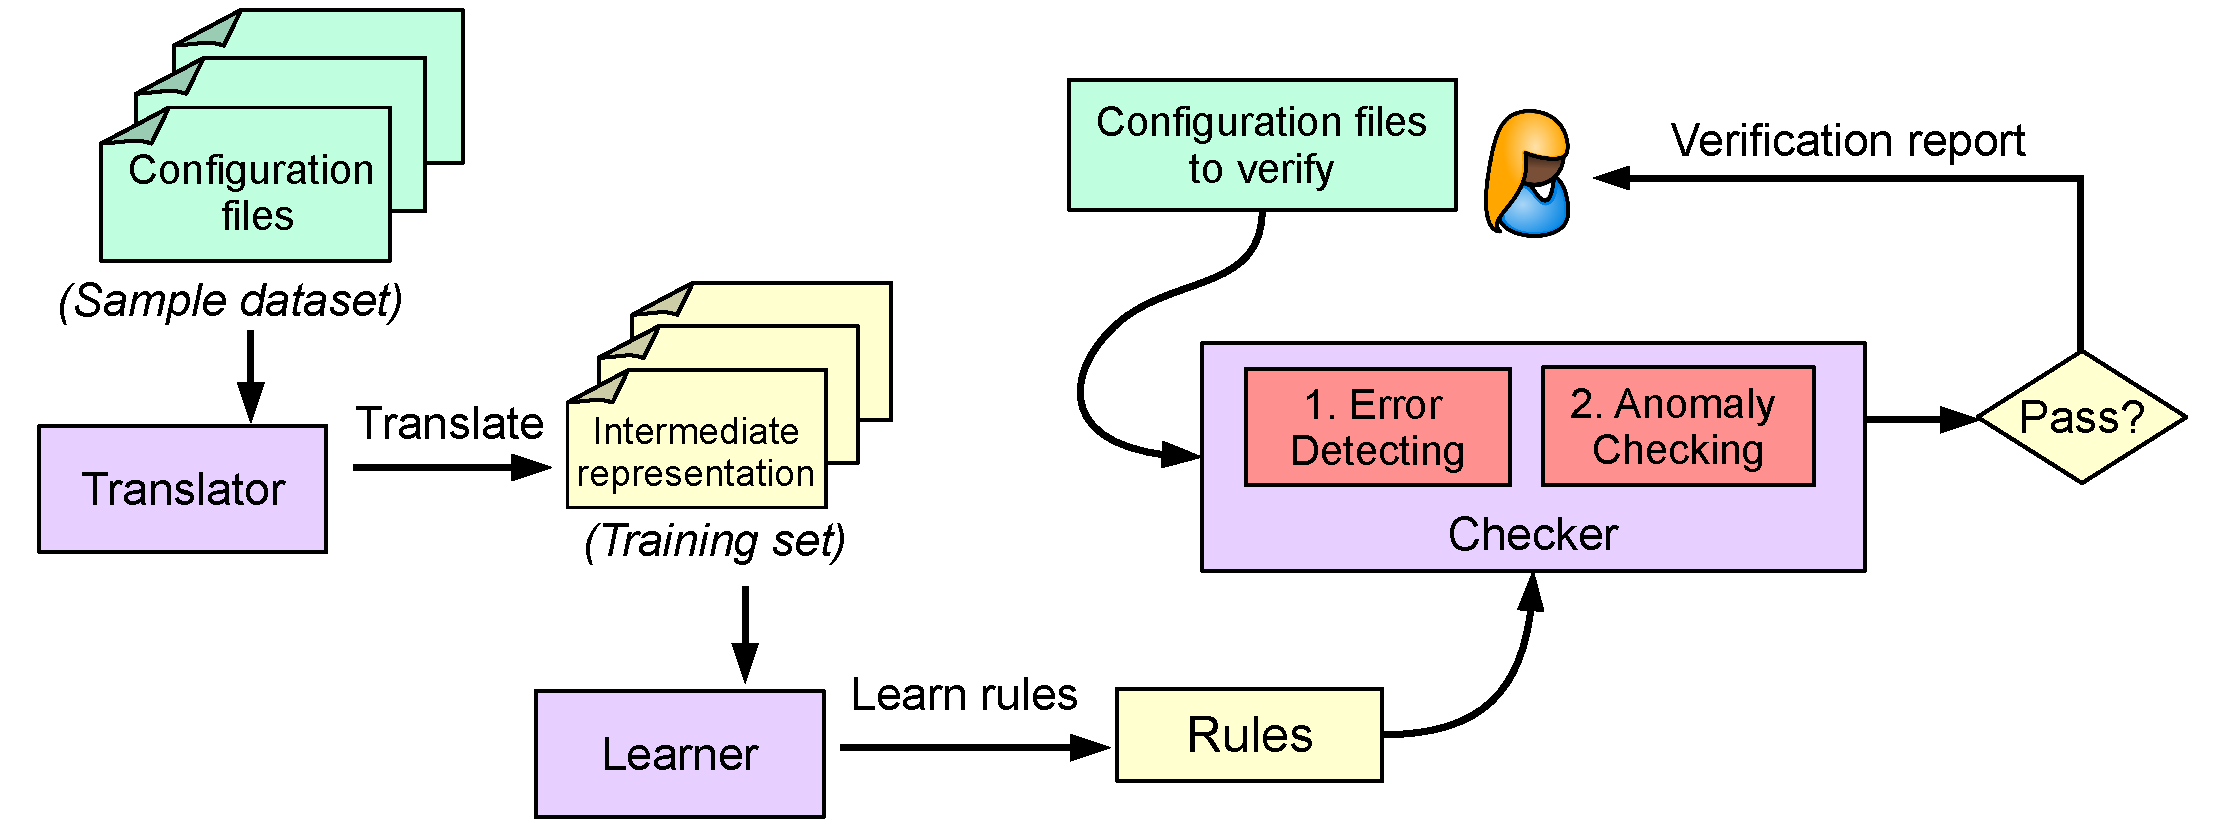
\includegraphics[width=0.9\textwidth]{figs/overview}
\caption{\app's workflow. The green components represent configuration 
  files, including both sample configuration datasets and users' input
  configuration files to verify. 
  The purple components are the modules of \app.
  Because template DB is not necessarily used, we use dashed
  arrow between it and the learner.
  Red boxes are sub-modules within the checker.
  The yellow components are results generated by \app's modules.}
\label{fig-overview}
\end{figure*}

\paragraph{Learning Specifications.}
Similarly as before, we start with an assumption 
that we are given a number of 
configuration files belonging to the same system (\eg, MySQL or Apache).
Additionally, we assume that files in this data set are 
not necessarily correct, but if there are errors they appear only in some
file. We then translate that dataset into a more structured
and typed intermediate representation, which follows
our defined language model (cf. Sec.~\ref{sec:lang}).
Since the type of an entry cannot be fully determined from 
the entry value, we introduce {\em probabilistic types}, which is
a more flexible type notion: to a indefinite keyword it 
assigns a list of possible types together with their probability 
distribution. The learner module employs a collection of learning
 algorithms to generate various rules and constraints.
It uses type-annotated templates to infer the rules. In addition, 
there are algorithms for detecting ordering errors and missing entry
errors, which do not depend on templates. However, this time, 
since the input set is not necessarily correct, the learned rules are
also annotated with the probability indicating the likelihood of being 
correct. 
 
 
potentially used to handle different types of configuration errors.
These rules and constraints are the outputs of the learner, 
and will be used by the checker to detect errors later.
Because the translator outputs probabilistically typed entries,
the learner is responsible for determining a type for each entry.

\com{Different from previous efforts, \eg, EnCore~\cite{zhang14encore},
which requires users or developers to provide explicit templates,
\app's learner encodes some predefined error-patterns 
to generate rules. 
As an illustration of a simple rule that we can learn,
consider an encoded pattern $X_1 \le X_2$, where $X_1$ and $X_2$ are
integer variables. The learner may derive the rule stating that
$\texttt{mysql.max\_persistent} \le \texttt{max\_connections}$. 
There is a classification and taxonomy of configuration errors in the 
existing work on automated configuration troubleshooting%
~\cite{yin11anempirical, configdataset}. 
Each class can be viewed as an error-pattern 
that \app should handle: we consider integer constraints, 
ordering errors, typing errors, correlation errors, etc.}

\com{
Although the learner has been capable of generating ruldoes not necessarily rely on templates,
\app still offers a database containing many templates,
as shown in Figure~\ref{fig-overview}.
Some of these templates are responsible for offering
specific system executional environment information.
A learning algorithm cannot derive rules 
related to environment violations, \eg,
whether the current account is 
the owner of a certain path, without information 
about the environment. 
In order to deal with comprehensive misconfiguration problems,
the learner needs a template DB to provide environment information,
thus detecting system environment-related configuration errors.}

\paragraph{Checking.}
The checker is used to detect rule violations in the configuration
files of interest. The inputs of the checker are the learned rules,
and the target configuration file to verify.
First, the checker translates the target configuration file into
the representation in our language model, and
then reports whether it has errors by checking it with the
learned rules. 
The checker generates a report (as shown in Sec.~\ref{sec:prelim}) about 
what errors the target configuration file has.
As shown in Figure~\ref{fig-overview},
there are two sub-modules in the checker. They are responsible for
checking rule violations and suspicious values, respectively.
In our experience, we found learned rules could be significantly reused
to check different configuration files, thus improving our usability.  
